% Define the document type and font size
\documentclass[12pt]{article}

\usepackage[spanish]{babel} % Package for the Spanish language
\usepackage[utf8]{inputenc} % Package for UTF-8 character encoding
\usepackage{geometry} % Package to configure document margins
\usepackage{graphicx} % Package to include graphics
\usepackage{listings} % Package to include source code in the document
\usepackage{xcolor} % Package to define colors
\usepackage{fancyhdr} % Package to customize headers and footers
\usepackage{amsmath} % Package for advanced mathematical symbols and environments
\usepackage{amssymb} % Package for additional mathematical symbols
\usepackage[hidelinks]{hyperref} % Package for hyperlinks in index and references (Keep this as the last package loaded)

\setlength{\parskip}{1em} % Space between paragraphs
\setlength{\parindent}{0.0in} % Indentation for paragraphs

% Definition of colors for source code
\definecolor{COLOR_COMMENTS}{HTML}{999999}
\definecolor{COLOR_KEYWORDS}{HTML}{37a5a6}
\definecolor{COLOR_IDENTIFIERS}{HTML}{ea76cb}
\definecolor{COLOR_STRINGS}{HTML}{ff7858}

% Configuration of the listings environment to display source code
\lstset{
frame=shadowbox,
aboveskip=3mm,
belowskip=3mm,
xleftmargin=10mm,
xrightmargin=10mm,
showstringspaces=false,
columns=flexible,
basicstyle={\footnotesize\ttfamily},
numbers=left,
numberstyle=\tiny\color{COLOR_COMMENTS},
keywordstyle=\color{COLOR_KEYWORDS},
stringstyle=\color{COLOR_STRINGS},
commentstyle=\color{COLOR_COMMENTS},
breaklines=true,
breakatwhitespace=true,
tabsize=4,
}

% Configuration of document margins
\geometry{
    a4paper,
    left=25mm,
    right=25mm,
    top=25mm,
    bottom=25mm
}
\graphicspath{{../img}} % Path for images

\title{Modelación Epidemiológica y Sistemas Dinámicos} % Document title
\author{María Laura Reina y Victoria Ruza} % Document author
\date{\today} % Document date

\begin{document}

    \begin{titlepage}
        \centering
        {
\includegraphics[width=0.2\textwidth]{logoBlack}\par}
        {\large {Universidad Central de Venezuela}\par}
        {\large {Facultad de Ciencias}\par}
        {\large {Escuela de Computación}\par}
        {\large {Cálculo Científico}\par}
        \vfill
        {\Huge {Modelación Epidemiológica y Sistemas Dinámicos}\par}
        \vfill
        {\large María Laura Reina y Victoria Ruza\par}
        \vspace{0.5cm}
        {\large \today\par}
    \end{titlepage}

    \pagenumbering{gobble}
    \tableofcontents
    \newpage
    \pagenumbering{arabic}

    \section{Objetivos}
        \subsection{Objetivo General}
            \begin{itemize}
                \item Implementar un modelo epidemiológico SEIR para simular la propagación de una enfermedad infecciosa en una población.
            \end{itemize}
        \subsection{Objetivos Específicos}
            \begin{itemize}
                \item Comprender y aplicar el método de Runge-Kutta de cuarto orden (RK4) para resolver sistemas de ecuaciones diferenciales.
                \item Analizar el impacto de diferentes escenarios de intervención en la propagación de la enfermedad.
                \item Evaluar el número reproductivo básico ($R_0$) y su influencia en la propagación de la enfermedad.
                \item Verificar la conservación de la población total durante la simulación y por tanto la validez del modelo.
            \end{itemize}
    \newpage

    \section{Metodología Numérica}
    Dado el modelo SEIR, se implementó el método de Runge-Kutta de cuarto orden (RK4) para resolver el sistema de ecuaciones diferenciales que describe la dinámica de la enfermedad. 
    
    Este método es conocido por su precisión y estabilidad en la resolución de sistemas dinámicos no lineales a comparación de métodos como Euler que a pesar de tener una implementación computacional más sencilla su poca precisión y acumulación de errores lo hacen una peor opción en cuanto a simulaciones precisas como la del modelado de una epidemia.

    \section{Implementación Computacional}
    La simulación del escenario comienza con la función \texttt{simulateSeir()} que recibe como argumentos el tipo de escenario (Libre o con intervención), la población total, los estados iniciales de la población, parámetros $\beta $(Probabilidad de transmisión), $\beta_{int}$ en caso de que el escenario sea de intervención, $\sigma$ (inverso del periodo medio de incubación) y $\gamma$ (inverso del periodo medio de infección), así como el tiempo total de simulación y el paso de tiempo (Cada cuánto se realiza una actualización sobre los estados).

    Inicializa el tiempo y los vectores de resultados para cada estado de la población, y luego itera sobre el tiempo, actualizando los estados de la población en cada paso utilizando el método RK4 descrito en el planteamiento del problema. Finalmente, devuelve los resultados de la simulación como una lista de flotantes \texttt{times} que representan los tiempos de cada actualización y una lista de arreglos de 4 elementos ([S, E, I, R]) \texttt{results} que representan los valores de los estados en cada momento.
        
    \newpage

    \section{Resultados y Análisis}
        \begin{figure}[h!]
            \centering
            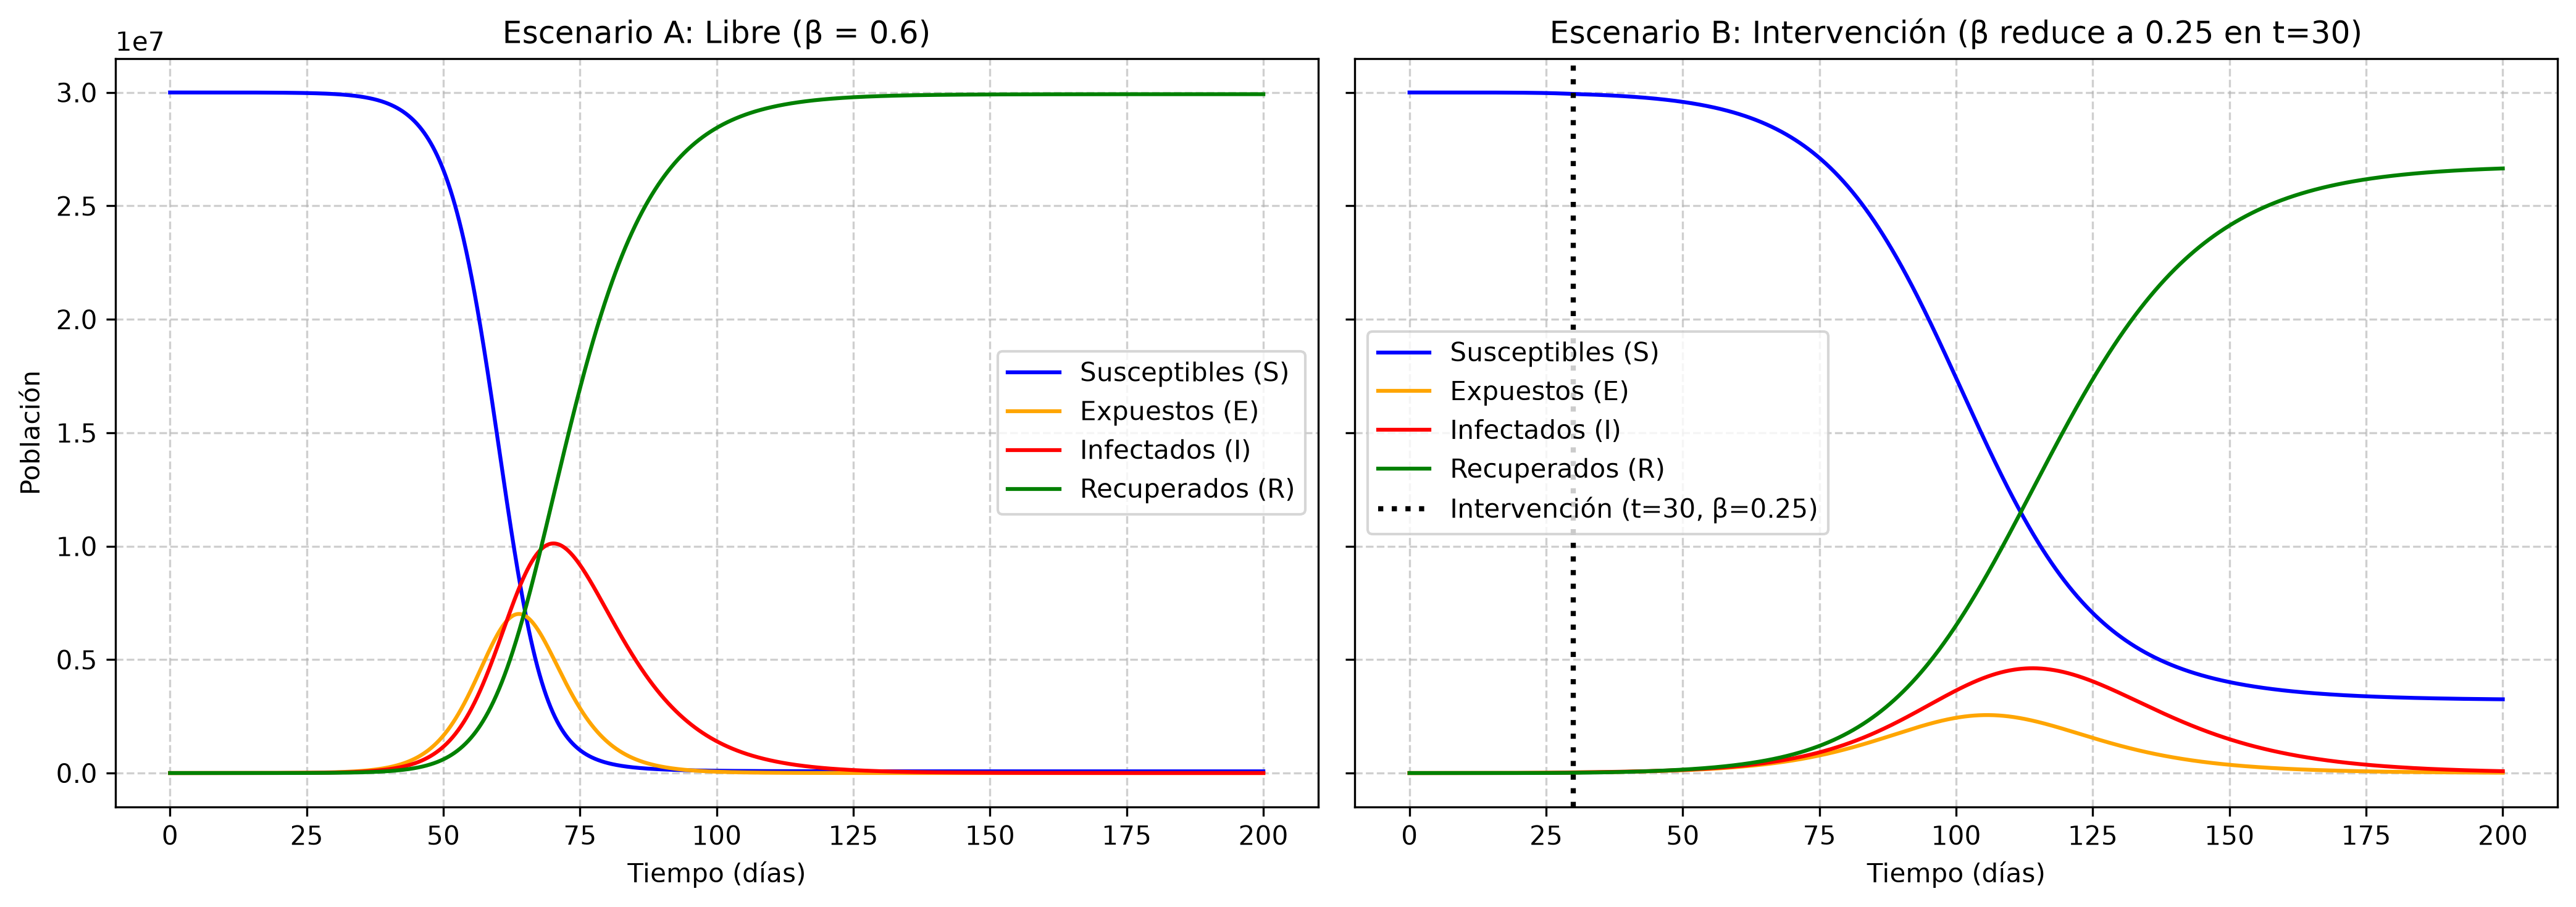
\includegraphics[width=1\textwidth]{EpidemiologicalModeling.png}
            \caption{Resultados de la simulación del modelo SEIR utilizando el método RK4.}
            \label{fig:seir_simulation}
        \end{figure}

        \subsection{Análisis del Umbral}
        El análisis del umbral se realiza calculando el número reproductivo básico (R0) para cada escenario. R0 se define como la relación entre la tasa de transmisión ($\beta$) y la tasa de recuperación ($\gamma$). Un R0 mayor que 1 indica que la enfermedad se propagará, mientras que un R0 menor que 1 indica que la enfermedad desaparecerá.

        \subsubsection*{Escenario A (Libre)}
        \begin{itemize}
            \item $R_0$ = 6.00
            \item Pico máximo de infectados: 10,120,571 personas
            \item Día del pico: 70.1 días
        \end{itemize}

        En el escenario A, el valor de $R_0$ puede ser interpretado como un indicador de la velocidad de propagación de la enfermedad. Un valor de 6.00 sugiere que cada persona infectada puede transmitir la enfermedad a 6 personas más en promedio, lo que resulta en un rápido aumento del número de casos produciendo un pico máximo de infectados en menor tiempo.

        \subsubsection*{Escenario B (Con Intervención $t >= 30$)}
        \begin{itemize}
            \item $R_0$ inicial ($t < 30$) = 6.00
            \item $R_0$ tras intervención ($t >= 30$) = 2.50
            \item Pico máximo de infectados: 4,619,246 personas
            \item Día del pico: 114.0 días
        \end{itemize}

        En cambio en el escenario B, la intervención comienza a tener efecto después de t = 30, lo que reduce el valor de $R_0$ a 2.50. Esto indica que la enfermedad se propaga a un ritmo significativamente más lento, produciendo no solo un menor número de infectados en el pico máximo y un retraso en el tiempo en que ocurre dicho pico, sino también una porción de la población que a pesar de ser suceptible no llega a infectarse debido a la extinción de la enfermedad.

        \subsection{Análisis de Conservación}

        La demostración numérica de la conservación de la población total se realiza verificando que la suma de los estados S, E, I y R permanezca constante a lo largo del tiempo. Esto se logra encontrando el máximo error absoluto entre la población total inicial y la suma de los estados en cada paso de tiempo. De manera que:

        \begin{itemize}
            \item Escenario A: $Error_{max} = 4.47\times10^{-8}$ personas (Aproximado a 2 decimales: 0.00)
            \item Escenario B: $Error_{max} = 8.20\times10^{-8}$ personas (Aproximado a 2 decimales: 0.00)
        \end{itemize}
        
        En ambos escenarios, el error máximo absoluto es extremadamente pequeño, lo que confirma que la población total se conserva durante la simulación.

    \newpage

    \section{Referencias}
    \begin{itemize}
        \item Begum, S., Mahmud, F., Hasan, M. Z., Kawsar, H. M. N., \& Akbar, M. A. (2026). A computationally efficient RK4-FNN hybrid approach for high-precision tuberculosis dynamics modeling: SIR/SEIR model applications. Arab Journal Of Basic And Applied Sciences, 33(1), 134-151. \newline \url{https://doi.org/10.1080/25765299.2026.2646030}
        \item mn6d Runge Kutta - Matemáticas y Métodos Numéricos. (2023). \newline \url{https://blogceta.zaragoza.unam.mx/mnumericos/unidad-6/mn6d/}
        \item Razapi, M. F. M., \& Mohamad, M. (2025). Comparison between the Runge Kutta Method and Euler Method for solving Dengue fever Disease model. \newline \url{https://periodical.uthm.edu.my/index.php/ekst/article/view/18524}
        \item Ridenhour, B., Kowalik, J. M., \& Shay, D. K. (2018). El número reproductivo básico (R0): consideraciones para su aplicación en la salud póblica. American Journal of Public Health, 108(S6), S455–S465. \newline \url{https://doi.org/10.2105/ajph.2013.301704s}
    \end{itemize}
\end{document}